\section{pbrt:系统概述}\label{sec:pbrt:系统概述}

pbrt是使用标准的\keyindex{面向对象}{object-oriented}{}技术构建的:
重要实体都定义了抽象\keyindex{基类}{base class}{class类}(例如
抽象基类\refvar{Shape}{}定义了所有几何形状必须实现的接口,
光源的抽象基类\refvar{Light}{}也有相似设计)。
系统大部分都是纯粹由这些抽象基类提供的接口来实现的;
例如检查光源与着色点之间遮挡物体的代码
调用\refvar{Shape}{}的相交方法
而不要考虑场景中出现的特定类型的形状。
这种方式使得扩展系统变得很容易,
新增一种形状只需要实现一个完成\refvar{Shape}{}接口的类并链接到系统。

pbrt用10个关键抽象基类写成,列于\reftab{1.1}。
向系统添加这些类的新实现很简单;
实现必须从适当的基类继承,
编译和链接到可执行文件,
且必须修改附录第\refchap{场景描述接口}中的对象创建例程
以创建解析场景描述文件所需要的对象。
\refsec{添加新物体的实现}
\sidenote{译者注:原书此处似乎链接错误,已纠正。}
将讨论这种扩展系统的方法的更多细节。


\begin{table}[h]
    \centering
    \begin{tabular}{l l l}
        \toprule
        \textbf{基类}         & \textbf{目录}           & \textbf{章节}                   \\
        \midrule
        \refvar{Shape}{}      & \ttfamily shapes/       & \refsec{基本形状接口}           \\
        \refvar{Aggregate}{}  & \ttfamily accelerators/ & \refsec{聚合}                   \\
        \refvar{Camera}{}     & \ttfamily cameras/      & \refsec{相机模型}               \\
        \refvar{Sampler}{}    & \ttfamily samplers/     & \refsec{采样接口}               \\
        \refvar{Filter}{}     & \ttfamily filters/      & \refsec{图像重构}               \\
        \refvar{Material}{}   & \ttfamily materials/    & \refsec{材质接口与实现}         \\
        \refvar{Texture}{}    & \ttfamily textures/     & \refsec{纹理接口与基本纹理}     \\
        \refvar{Medium}{}     & \ttfamily media/        & \refsec{介质}                   \\
        \refvar{Light}{}      & \ttfamily lights/       & \refsec{光源接口}               \\
        \refvar{Integrator}{} & \ttfamily integrators/  & \refsub{积分器接口与采样积分器} \\
        \bottomrule
    \end{tabular}
    \caption{主要接口类型。pbrt大部分由此处列出的10个关键抽象基类实现。
        每个的实现都很容易添加到系统中扩展其功能。}
    \label{tab:1.1}
\end{table}

pbrt源码发布于\href{https://pbrt.org/}{\ttfamily pbrt.org}。
(大量场景示例\footnote{\url{http://pbrt.org/scenes-v3.html}}也可分开下载。)
所有的pbrt核心代码均在目录{\ttfamily src/core}内,
函数\refvar{main}{()}在
短文件\href{https://github.com/mmp/pbrt-v3/tree/master/src/main/pbrt.cpp}{\ttfamily main/pbrt.cpp}内。
抽象基类实例的各种实现在分开的目录下:
{\ttfamily src/shapes}有基类\refvar{Shape}{}的实现,
{\ttfamily src/materials}有基类\refvar{Material}{}的实现,以此类推。

本节有许多pbrt扩展版本渲染的图像。
其中从\reffig{1.11}到\reffig{1.14}
\sidenote{译者注:原书\reffig{1.14}引用文献似乎遗漏了链接,推测是\citep{10.1145/74333.74361}。}
都引人瞩目:
它们不仅令人过目不忘,而且每张都是渲染课程的学生在
最后的课程作业中对pbrt扩展新功能渲染得到的有趣图像。
这些是课程中最佳图像的一部分。
\begin{figure}[ht]
    \centering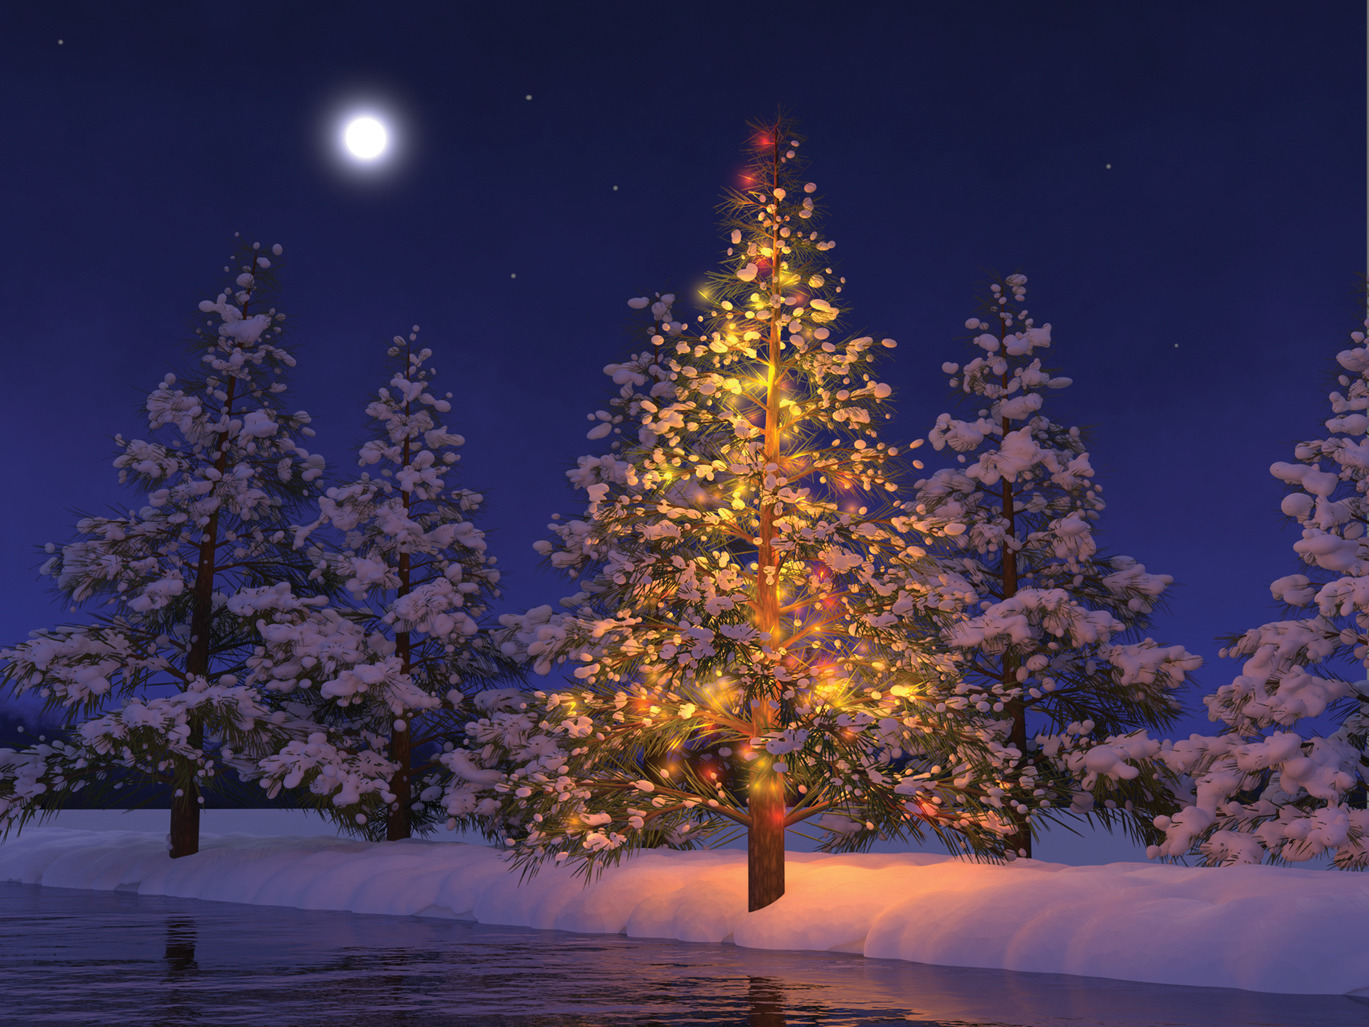
\includegraphics[width=\linewidth]{chap01/nightsnow.jpg}
    \caption{Guillaume Poncin和Pramod Sharma用许多方法扩展了pbrt,
        实现了一系列复杂渲染算法,
        制作出这张斯坦福大学CS348b渲染竞赛获奖图像。
        树木由L系统程序化建模,
        辉光图像处理滤波器增加了树上灯光的真实感,
        雪由metaball程序化建模,
        次表面散射算法考虑了光在离开雪前在雪下传播了一段距离的影响,
        赋予了雪逼真的外观。}
    \label{fig:1.11}
\end{figure}
\begin{figure}[ht]
    \centering
\includegraphics[width=\linewidth]{chap01/icecave.png}
    \caption{Abe Davis、David Jacobs和Jongmin Baek渲染了这张惊艳的冰窟图像,
        夺得2009斯坦福大学CS348b渲染竞赛大奖。
        他们首先实现了对冰川作用,即雪多年落下、融化、再冻结形成分层冰层这一物理过程的仿真。
        然后他们模拟了融水径流对冰的侵蚀,生成了冰的几何模型。
        体积内的光散射由体积光子映射模拟;
        冰的蓝色完全取决于在冰体中对依赖于波长的光吸收的建模。}
    \label{fig:1.12}
\end{figure}
\begin{figure}[ht]
    \centering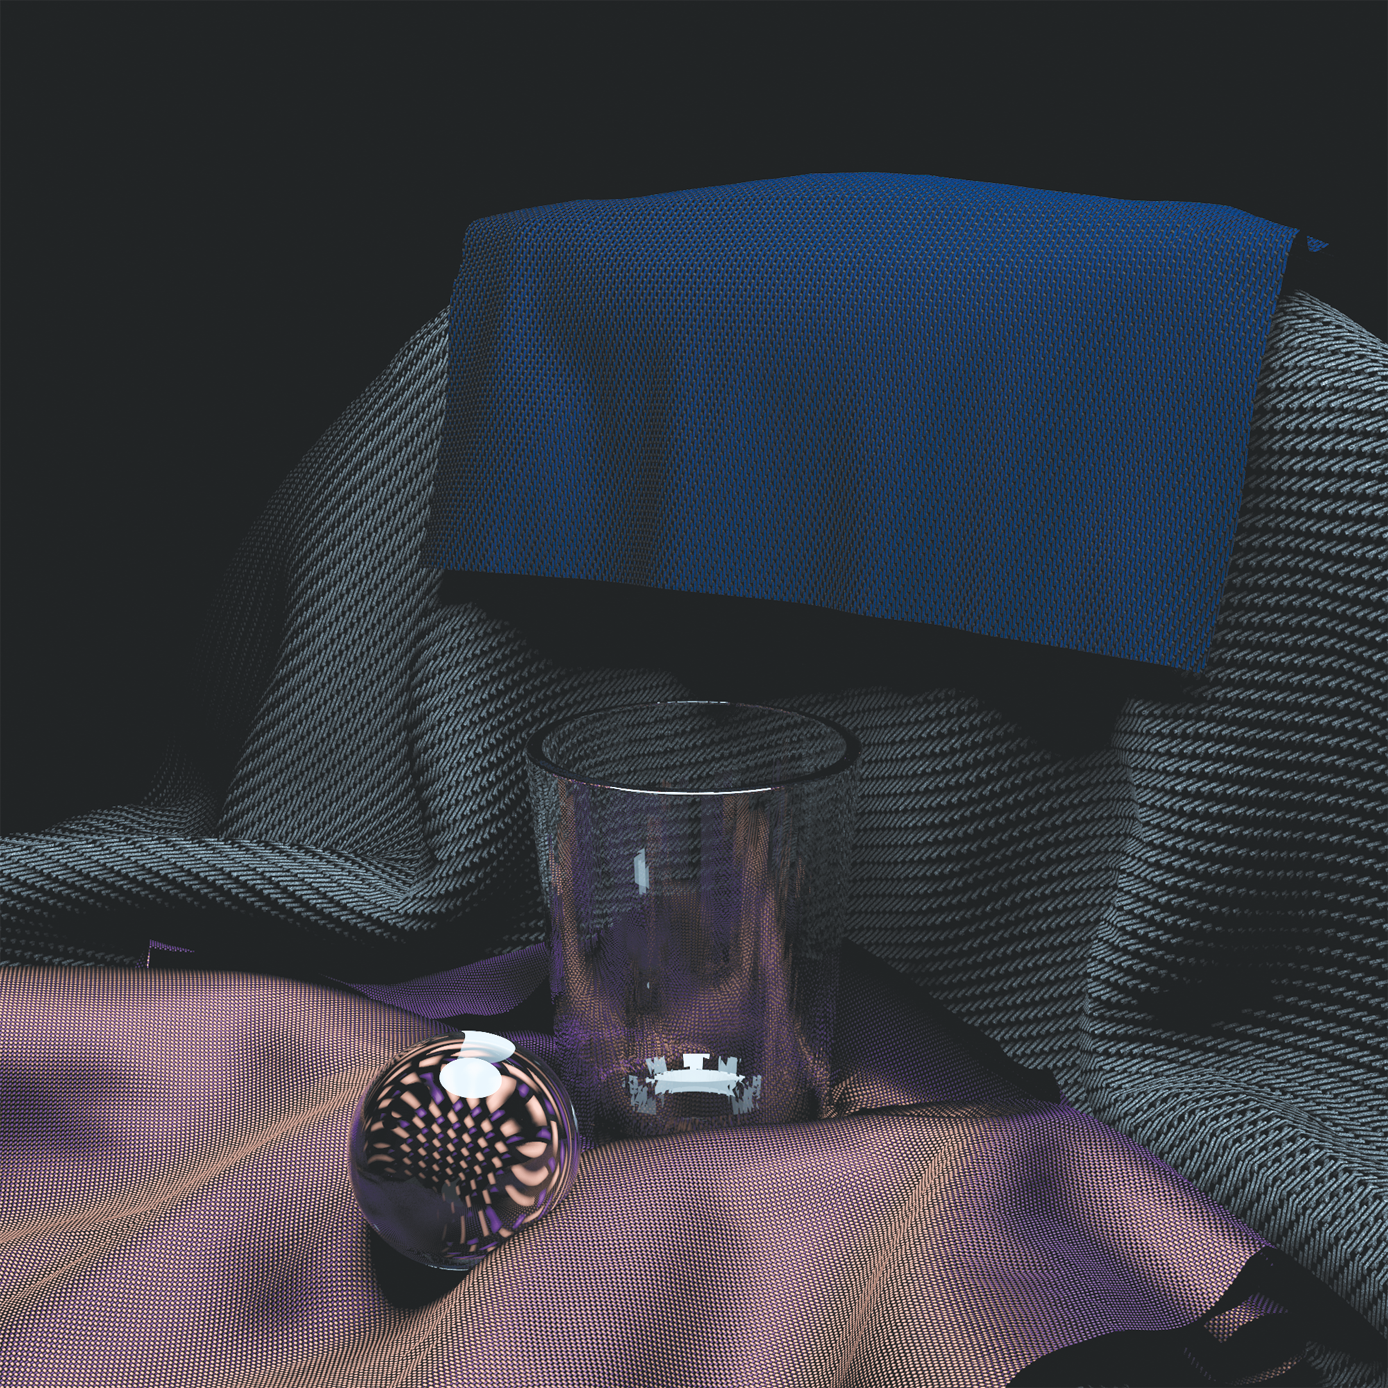
\includegraphics[width=\linewidth]{chap01/cloth.png}
    \caption{Lingfeng Yang实现了双向纹理函数来模拟布料的外观,
        添加了解析的自阴影模型,
        渲染了这张2009斯坦福大学CS348b渲染竞赛一等奖图像。}
    \label{fig:1.13}
\end{figure}

\subsection{执行阶段}\label{sub:执行阶段}

pbrt在概念上可分为两个执行阶段。
首先,解析用户提供的场景描述文件。
场景描述是一个文本文件,
指定了构成场景的几何形状及其材质属性、
对其照明的光源、虚拟相机在场景中的摆放位置、
整个系统所用的各个算法的参数等。
输入文件的每个语句都直接映射到
附录第\refchap{场景描述接口}
\sidenote{译者注:原书此处似乎链接错误,已纠正。}
中的一个例程;
这些例程包含了描述场景的程序接口。
场景文件格式的文档详见pbrt网站\href{https://pbrt.org/}{pbrt.org}。

\begin{figure}[ht]
    \centering\includegraphics[width=\linewidth]{chap01/furrydog.png}
    \caption{Jared Jacobs和Michael Turitzin为pbrt增加了
        Kajiya和Kay基于纹素的毛发渲染算法\citep{10.1145/74333.74361}并渲染了该图像,
        狗毛和粗毛地毯都是用纹素毛发算法渲染的。}
    \label{fig:1.14}
\end{figure}


\subsection{场景表示}\label{sub:场景表示}

\begin{lstlisting}
`\initcode{Main program}{=}`
int `\initvar{main}{}`(int argc, char *argv[]) {
    Options options;
    std::vector<std::string> filenames;
    `\refcode{Process command-line arguments}{}` 
    `\refvar{pbrtInit}{}`(options);
    `\refcode{Process scene description}{}` 
    `\refvar{pbrtCleanup}{}`();
    return 0;
}
\end{lstlisting}

\subsection{积分器接口与采样积分器}\label{sub:积分器接口与采样积分器}

\begin{lstlisting}
`\initcode{Integrator Declarations}{=}`
class `\initvar{Integrator}{}` {
public:
    `\refcode{Integrator Interface}{}`
};
\end{lstlisting}